\begin{table}[tb]
\centering
\caption{Main comparisons between methods per backbone. Each entry is the held-out AUROC (classification) or Dice (segmentation) of the first method minus that of the second, averaged over labels or structures, with the 95\% bootstrap interval over cohorts, labels and cases in brackets, which does not include seed variation (Appendix~\ref{app:stats}). The $>0$ columns count the cohorts (datasets) with a positive mean difference. Lin and Attn denote the frozen linear and attentive probes and Dec the frozen multi-depth decoder; Joint $-$ per-task compares one model per cohort with one model per label and averages over methods. Each label's per-task and joint values are averaged, except in the two LoRA $-$ Dec sub-rows. Pooled estimates are in Table~\ref{tab:cis}. $^\dagger$Includes runs that did not train (Section~\ref{sec:setup}).}
\label{tab:key}
\vspace{-6pt}
\renewcommand{\mci}[3]{#1\,{\scriptsize[#2, #3]}}\adjustbox{max width=\textwidth}{\small\setlength{\tabcolsep}{3.5pt}
\begin{tabular}{@{}lcccccc@{\hspace{10pt}}lcccc@{}}
\toprule
\multicolumn{7}{c}{\textit{Classification} (AUROC)} & \multicolumn{5}{c}{\textit{Segmentation} (Dice)} \\
\cmidrule(r){1-7}\cmidrule(l){8-12}
 & \multicolumn{2}{c}{TAP-CT} & \multicolumn{2}{c}{SPECTRE} & \multicolumn{2}{c}{Pillar-0} & & \multicolumn{2}{c}{TAP-CT} & \multicolumn{2}{c}{SPECTRE} \\
\cmidrule(lr){2-3}\cmidrule(lr){4-5}\cmidrule(lr){6-7}\cmidrule(lr){9-10}\cmidrule(lr){11-12}
Comparison & Mean & $>0$ & Mean & $>0$ & Mean & $>0$ & Comparison & Mean & $>0$ & Mean & $>0$ \\
\midrule
LoRA $-$ Lin & \mci{$+0.032$}{$+0.007$}{$+0.053$} & 4/5 & \mci{$+0.037$}{$+0.009$}{$+0.075$} & 4/4 & \mci{$+0.033$}{$+0.021$}{$+0.044$} & 1/1 & Dec $-$ Lin & \mci{$+0.085$}{$+0.055$}{$+0.109$} & 5/5 & \mci{$+0.061$}{$+0.027$}{$+0.088$} & 5/5 \\
LoRA $-$ Attn & \mci{$+0.022$}{$+0.006$}{$+0.042$} & 5/5 & \mci{$+0.033$}{$+0.003$}{$+0.078$} & 4/4 & \mci{$+0.034$}{$+0.021$}{$+0.052$} & 1/1 & LoRA $-$ Dec & \mci{$-0.005$}{$-0.021$}{$+0.024$} & 4/5 & \mci{$+0.023$}{$-0.018$}{$+0.076$} & 4/5 \\
Attn-only FT $-$ LoRA & \mci{$+0.019$}{$-0.001$}{$+0.054$} & 4/5 & \mci{$+0.002$}{$-0.037$}{$+0.026$} & 2/4 & \mci{$+0.001$}{$-0.002$}{$+0.004$} & 1/1 & \quad per-structure & \mci{$-0.021$}{$-0.036$}{$+0.002$} & 2/5 & \mci{$+0.006$}{$-0.003$}{$+0.031$} & 5/5 \\
Full FT $-$ Lin & \mci{$+0.022$}{$-0.061$}{$+0.068$} & 4/5 & \mci{$-0.117^{\dagger}$}{$-0.195$}{$-0.059$} & 0/4 & \mci{$+0.004$}{$-0.013$}{$+0.021$} & 1/1 & \quad joint & \mci{$+0.011$}{$-0.021$}{$+0.066$} & 4/5 & \mci{$+0.040$}{$-0.039$}{$+0.147$} & 4/5 \\
 &  &  &  &  &  &  & Full FT $-$ Dec & \mci{$0.000$}{$-0.024$}{$+0.016$} & 4/5 & \mci{$-0.003$}{$-0.035$}{$+0.009$} & 2/5 \\
\cmidrule(r){1-7}\cmidrule(l){8-12}
Joint $-$ per-task & \mci{$+0.012$}{$-0.014$}{$+0.038$} & 3/5 & \mci{$-0.003$}{$-0.044$}{$+0.051$} & 3/4 & \mci{$-0.008$}{$-0.013$}{$-0.001$} & 0/1 & Joint $-$ per-task & \mci{$-0.046$}{$-0.090$}{$-0.008$} & 0/5 & \mci{$-0.058$}{$-0.093$}{$-0.009$} & 0/5 \\
\bottomrule
\end{tabular}
}
\end{table}

Table~\ref{tab:key} summarizes the main comparisons; per-label results, paired tests, seed repeats and controls, and success and failure cases are given in Appendices~\ref{app:perlabel}, \ref{app:paired}, \ref{app:revision} and~\ref{app:cases}.

\subsection{Classification}
\label{sec:clsres}

\begin{figure}[tb]
\centering
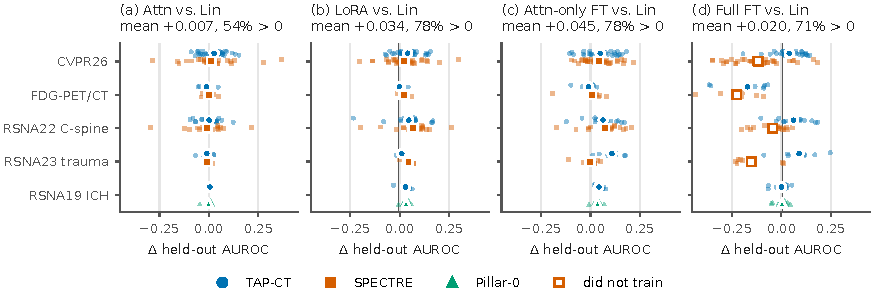
\includegraphics[width=\textwidth]{figures/fig_cls.pdf}
\vspace{-8pt}
\caption{Per-label change in held-out AUROC relative to the linear probe of the same backbone, cohort and training mode, for (a) the frozen attentive probe, (b) LoRA and (c) attention-only fine-tuning. Small markers denote individual label--mode pairs and large markers the mean per cohort. Panel titles give the mean change and the share of pairs above zero over all backbones. All methods, including full fine-tuning, are shown in Figure~\ref{fig:methods}.}
\label{fig:cls}
\end{figure}

\begin{figure}[tb]
\centering
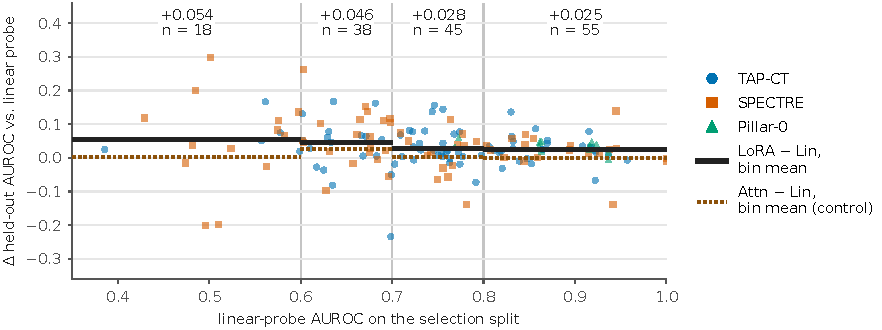
\includegraphics[width=\textwidth]{figures/fig_gain_vs_probe.pdf}
\vspace{-8pt}
\caption{Gain of LoRA over the linear probe in held-out AUROC, per label--mode pair, against the linear probe's selection-split AUROC (marker shape: backbone). Horizontal segments give bin means over all backbones, with bin edges at 0.6, 0.7 and 0.8. The dotted segments show the same bin means for the frozen attentive probe, as a negative control. Above each bin, the LoRA mean, the attentive-probe mean (brown) and the number of pairs are printed.}
\label{fig:gainprobe}
\end{figure}

Across TAP-CT, SPECTRE and Pillar-0, adapting the encoder with LoRA improved held-out AUROC over both frozen probes, by \magn{\numCiClsloralinAllMeandiff} over the linear probe and by \magn{\numCiClsloraattnAllMeandiff} over the frozen attentive probe, which uses the same head (Table~\ref{tab:cis}; per backbone in Table~\ref{tab:key} and Figure~\ref{fig:cls}). Both 95\% intervals exclude zero, and the improvement over the attentive probe was positive in all \numCiClsloraattnAllClustersN{} cohort--backbone pairs. The mean held-out AUROC rose from \pooledtapctlin{} to \pooledtapctlora{} on TAP-CT, from \pooledspectrelin{} to \pooledspectrelora{} on SPECTRE and from \pooledpillarZlin{} to \pooledpillarZlora{} on Pillar-0 (Table~\ref{tab:headline}). Fine-tuning all parameters of the attention modules showed the same pattern, with gains of \magn{\numCiClsattnftlinAllMeandiff} and \magn{\numCiClsattnftattnAllMeandiff}, respectively (Table~\ref{tab:cis}). In contrast, the frozen attentive probe improved on the linear probe by only \magn{\numCiClsattnlinAllMeandiff}, which suggests that the gain stems from adapting the encoder rather than from the head. As shown in Figure~\ref{fig:gainprobe}, the gain was largest for labels on which the linear probe performed worst (\magn{\numGainbinLowMeandiff} at a selection AUROC of at most 0.6, against \magn{\numGainbinTopMeandiff} above 0.8). Moreover, the gain persisted after excluding FDG-PET/CT and COVID-CTset, whose labels may be predictable from the acquisition rather than the anatomy (\magn{\numCiClsloralinnoscAllMeandiff}; Table~\ref{tab:cis}). LoRA also outperformed the linear probe in \numSeedsclsLoraLinAllPosN{} of \numSeedsclsLoraLinAllPairsN{} cohort--seed pairs of the repeated joint models (Table~\ref{tab:seedscls}).

At the default settings, fine-tuning all attention parameters achieved the best mean rank over all label--mode pairs (\numRankAttnftMean{}, against \numRankLoraMean{} for LoRA; Figure~\ref{fig:overview}c) and ranked above LoRA on every backbone. It outperformed LoRA in \numSeedsclsAttnftLoraAllPosN{} of \numSeedsclsAttnftLoraAllPairsN{} cohort--seed pairs of the repeated joint models and by \magn{\numCiClsattnftloraAllMeandiff} on average over the main runs, although this interval includes zero (Table~\ref{tab:cis}); the difference was largest on TAP-CT (\magn{\numCiClsattnftloraTapctMeandiff}). LoRA updates \numParamsratioPillarZAttnftLora{} to \numParamsratioSpectreAttnftLora{} times fewer encoder parameters (Figure~\ref{fig:arms}c), yet this did not make training cheaper. Its peak GPU memory per step was within \numCostClsLoraAttnftMaxGibdiff{}\,GiB of that of attention-only fine-tuning on every backbone and its steps were not faster (Table~\ref{tab:cost}), so the saving lies in the encoder weights stored per model. Fine-tuning the MLP weights instead of the attention weights performed on par with attention-only fine-tuning on TAP-CT and Pillar-0, but remained behind it by \magn{\numCtrlSpectreMlpftAttnftMeandiff} on SPECTRE (joint models; Table~\ref{tab:controls}).

Full fine-tuning required its own setting. With the default setting, it was ahead of the linear probe on TAP-CT by \magn{\numCiClsfullftlinTapctMeandiff} on average, with an interval that includes zero (Table~\ref{tab:key}), and was the best joint model on RSNA23 trauma (Table~\ref{tab:cls}), where \citet{liu2025anymc3d} also found full fine-tuning ahead of LoRA for spleen injury. On Pillar-0 it performed on par with the linear probe, whereas on SPECTRE it did not train: its median selection AUROC remained at \numTrajSpectrefullftLast{}, against \numTrajSpectreattnftLast{} for attention-only fine-tuning at the same learning rates (Figure~\ref{fig:fullftspectre}). With layer-wise learning-rate decay of 0.75 per block, the best of three alternative settings on selection data, SPECTRE Full FT trained and was ahead of LoRA by \magn{\numFixselSpectreLoraMeandiff} in the joint models (Table~\ref{tab:fullftfix}). However, this comparison favors full fine-tuning, as LoRA was not re-tuned.

On average over backbones, none of the LoRA variants improved on plain LoRA by more than \magn{\numVsloraAllBabmilMeandiff} (Figure~\ref{fig:methods}). The two-stage schedules and rsLoRA were behind LoRA by \magn{\numVsloraAllLinThenLoragMeandiff} to \magn{\numVsloraAllAttnThenLoragMeandiff}. At a quarter of the learning rate, which matches its update scale to that of LoRA, rsLoRA performed on par with LoRA on SPECTRE and Pillar-0 but remained behind it on TAP-CT by \magn{\numCtrlTapctRsloraLowlrLoraMeandiff} (Table~\ref{tab:controls}). These rankings hold for one default setting and 8000 steps per method. On CVPR26, a 26\,000-step schedule changed the joint models by $\numJointlongTapctMindiff$ to $\numJointlongTapctMaxdiff$ on TAP-CT and by $\numJointlongSpectreMindiff$ to $\numJointlongSpectreMaxdiff$ on SPECTRE, depending on the method (Table~\ref{tab:ladder}), which is as large as the differences between methods.

\subsection{Segmentation}
\label{sec:segres}

Replacing the linear probe by the frozen multi-depth decoder improved Dice on every dataset and backbone, by \magn{\numSegdeltaTapctLinDecMeandiff} on TAP-CT and \magn{\numSegdeltaSpectreLinDecMeandiff} on SPECTRE (Table~\ref{tab:key}; examples in Figure~\ref{fig:examplesseg}, Appendix~\ref{app:cases}). On TAP-CT, this accounted for all of the gain of LoRA over the linear probe (\magn{\numSegdeltaTapctLinLoraMeandiff}), and on SPECTRE for most of it (\magn{\numSegdeltaSpectreLinLoraMeandiff}). The pretrained weights nonetheless mattered, as the TAP-CT architecture trained from a random initialization was behind fine-tuning of the pretrained encoder at the same budget on every dataset, by \magn{\numScratchLitsTapctMeandiff} to \magn{\numScratchTotalsegTapctMeandiff} Dice (Table~\ref{tab:scratch}).

On top of the decoder, adapting the encoder changed Dice little on average. LoRA changed Dice relative to the frozen decoder by $\numCiSegloradecTapctMeandiff$ on TAP-CT and $\numCiSegloradecSpectreMeandiff$ on SPECTRE, with intervals that include zero (Table~\ref{tab:key}, Figure~\ref{fig:key}; per-structure changes in Figure~\ref{fig:seg}, Appendix~\ref{app:paired}). Its largest gain occurred where the frozen decoder was weakest, in the SPECTRE AMOS22 joint model (\numSegAmosBBSpectreJointDec{} to \numSegAmosBBSpectreJointLora{}; Table~\ref{tab:segbudget}). Full fine-tuning achieved the best mean rank (\numSegrankFullftMean{}, against \numSegrankLoraMean{} for LoRA; Figure~\ref{fig:overview}e), driven by its rank on TAP-CT (\numSegrankTapctFullftMean{}). However, its mean change on TAP-CT was $\numSegdeltaTapctDecFullftMeandiff$, because \numSegdeltaTapctDecFullftDropN{} structure--mode pairs lost more than 0.1, among them the AMOS22 esophagus of the joint model ($\numSegdeltaTapctDecFullftMindiff$; Appendix~\ref{app:cases}). In addition, tripling the steps of the 15-structure joint models improved their Dice by \magn{\numSegbudgetgainTapctMeandiff} on TAP-CT and \magn{\numSegbudgetgainSpectreMeandiff} on SPECTRE (Table~\ref{tab:segbudget}), and \numConvSegAllLateBetter\% of segmentation runs selected one of their last two validations (Figure~\ref{fig:segconv}). These comparisons therefore rank methods at a fixed budget rather than at convergence.

\begin{figure}[tb]
\centering
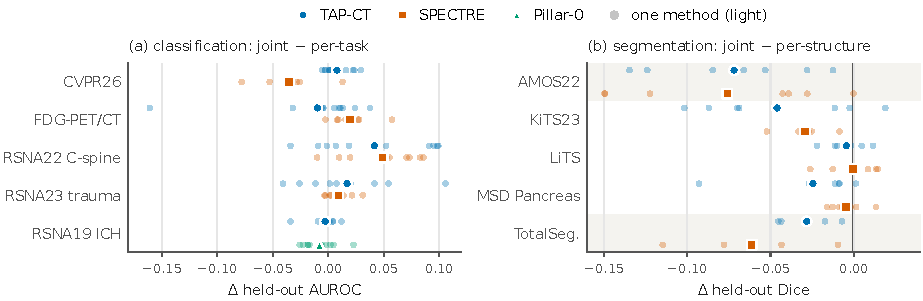
\includegraphics[width=\textwidth]{figures/fig_joint_main.pdf}
\vspace{-14pt}
\caption{Joint minus per-task training. (a) Joint minus per-task held-out AUROC per classification cohort and (b) joint minus per-structure held-out Dice per segmentation dataset. Large markers denote the mean over methods and labels (structures) per backbone, and light markers, in the backbone's color, individual methods. Shaded rows mark the 15-structure datasets, whose joint models were trained for 24\,000 steps. Values right of zero favor one joint model per dataset. Per-label values are given in Appendix~\ref{app:perlabel} and Figure~\ref{fig:joint}.}
\label{fig:jointmain}
\end{figure}

\subsection{Per-task and Joint Training}
\label{sec:jointres}

In classification, one joint model per cohort performed on par with one model per label on average, at a fraction of the training. Joint minus per-task AUROC was $\numCiClsjointAllMeandiff$ over TAP-CT, SPECTRE and Pillar-0 (interval $\numCiClsjointAllLodiff$ to $\numCiClsjointAllHidiff$; Table~\ref{tab:cis}), whereas a joint model uses $1/K$ of the training steps of the $K$ per-label models it replaces. On Pillar-0 alone, the joint models were slightly behind ($\numCiClsjointPillarZMeandiff$, interval $\numCiClsjointPillarZLodiff$ to $\numCiClsjointPillarZHidiff$). Per cohort and averaged over methods, the difference ranged from $\numJointdeltaMin$ to $\numJointdeltaMax$ (Figure~\ref{fig:jointmain}a; per method in Figure~\ref{fig:joint}).

\label{sec:jointseg}In segmentation, in contrast, the joint models lost Dice, mostly on small structures and partly through the smaller budget per structure. With each structure counted once (Table~\ref{tab:key}), one joint model per dataset changed Dice by $\numCiSegjointTapctMeandiff$ on TAP-CT and $\numCiSegjointSpectreMeandiff$ on SPECTRE, most on the 15-structure AMOS22 (Figure~\ref{fig:jointmain}b). Averaged over structure--method pairs, the joint model lost \magn{\numSegjointTapctMeandiff} Dice on TAP-CT and \magn{\numSegjointSpectreMeandiff} on SPECTRE. Much of this loss came from \numSegcollapseN{} of \numSegcollapseCellsN{} pairs on small structures, namely the adrenal glands and esophagus of AMOS22 and the merged glands of TotalSegmentator, on which the joint model scored below 0.01. Excluding these pairs, the losses were \magn{\numSegjointTapctNocollapseMeandiff} and \magn{\numSegjointSpectreNocollapseMeandiff}, respectively. Training crops are centered on a random foreground voxel of all structures together, so small structures rarely lie at the center of a crop; we did not test structure-balanced sampling \citep{isensee2021nnunet}. At matched total compute, with each per-structure model trained for 1600 steps, the joint frozen decoder and joint full fine-tuning remained behind per-structure models in three of the four pairs (Table~\ref{tab:segcm}). The joint LoRA model, in contrast, outperformed per-structure LoRA by \magn{\numCmTotalsegSpectreLoraJointdiff} to \magn{\numCmAmosBBSpectreLoraJointdiff} Dice, but per-structure LoRA at 1600 steps reached only \numCmAmosBBTapctLoraMatchedMean{} to \numCmTotalsegSpectreLoraMatchedMean{} Dice, against \numCmAmosBBSpectreDecMatchedMean{} to \numCmTotalsegSpectreDecMatchedMean{} for per-structure decoders. The smaller budget per structure therefore explains part, but not all, of the loss of the joint models.
